% description distribution methode aleatoire
% expliquer les distributions moy_dh et moy_dl  et les courbes de ces distributions pour une methode de correction
% interpretation selon loi uniforme  pour p = 0.5
% k = [0,5] : une figure
% k = [6,9] : une autre figure
% k = [10,50] : une autre figure
% cas particulier pour la loi de poisson

%\begin{figure}[htb!] 
%\centering
%%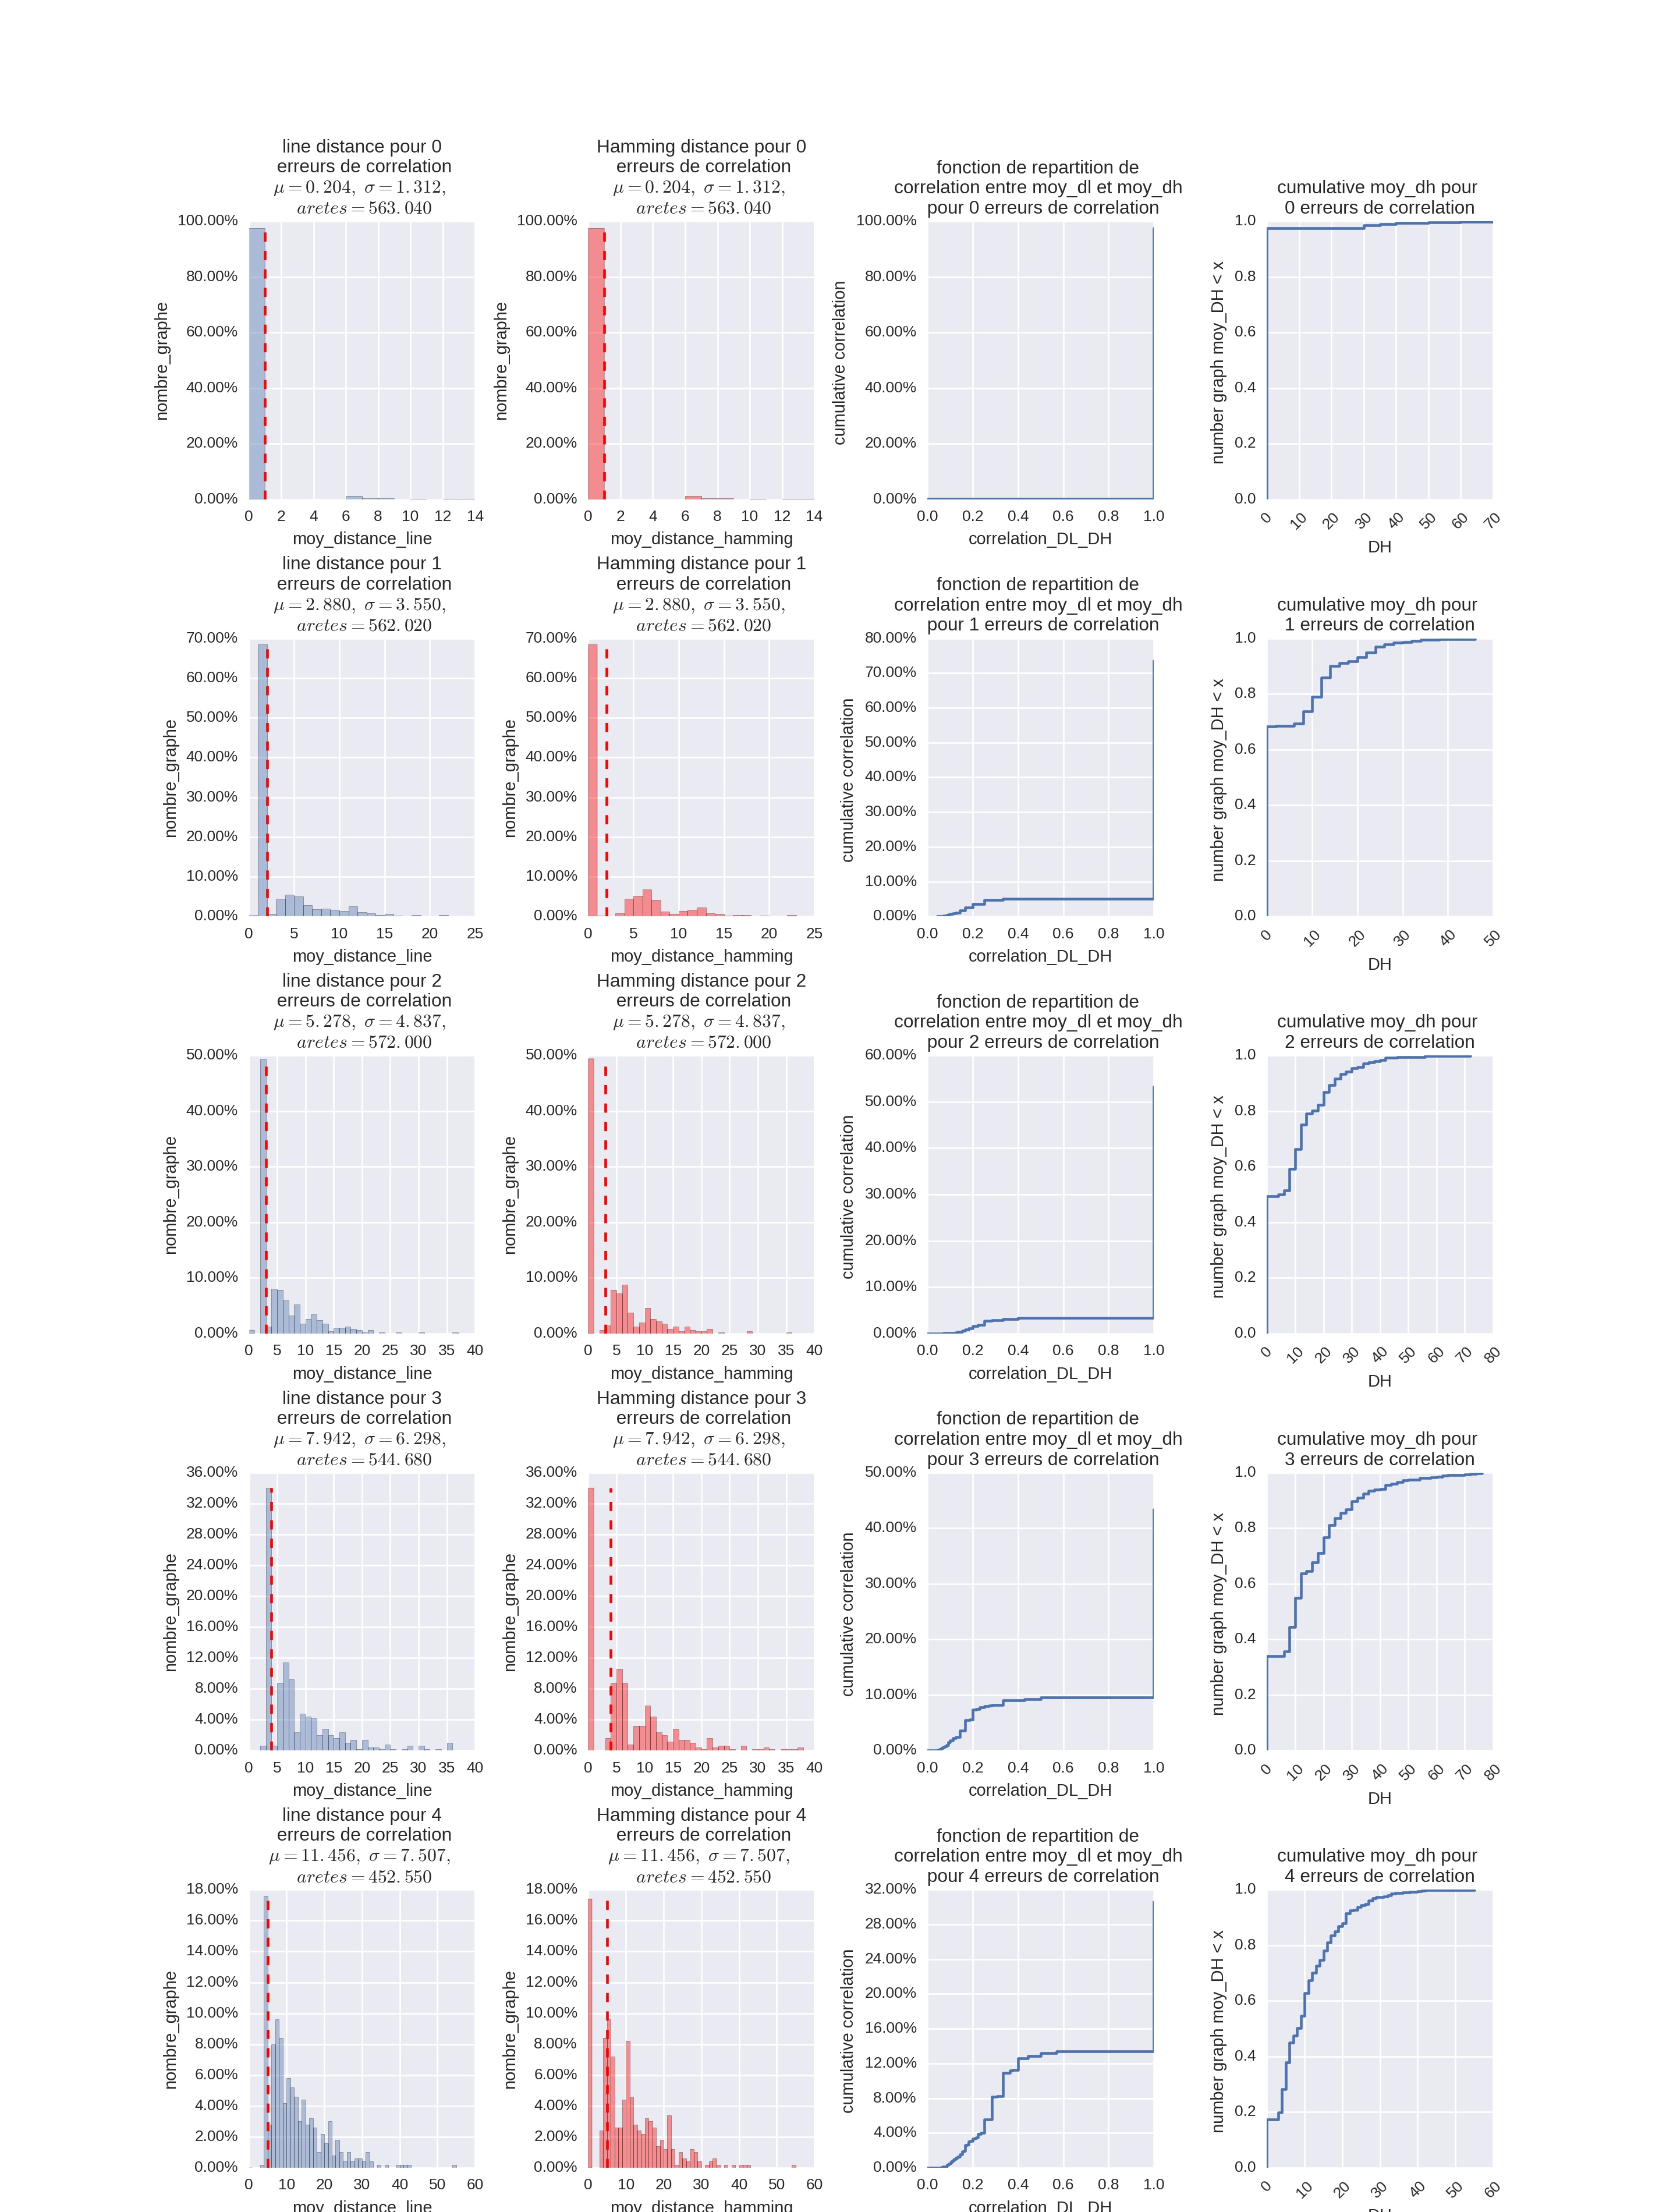
\includegraphics[scale=0.150]{permut_distanceMoyenDLDH_k_0_4_aleatoire_p_05.jpeg}
%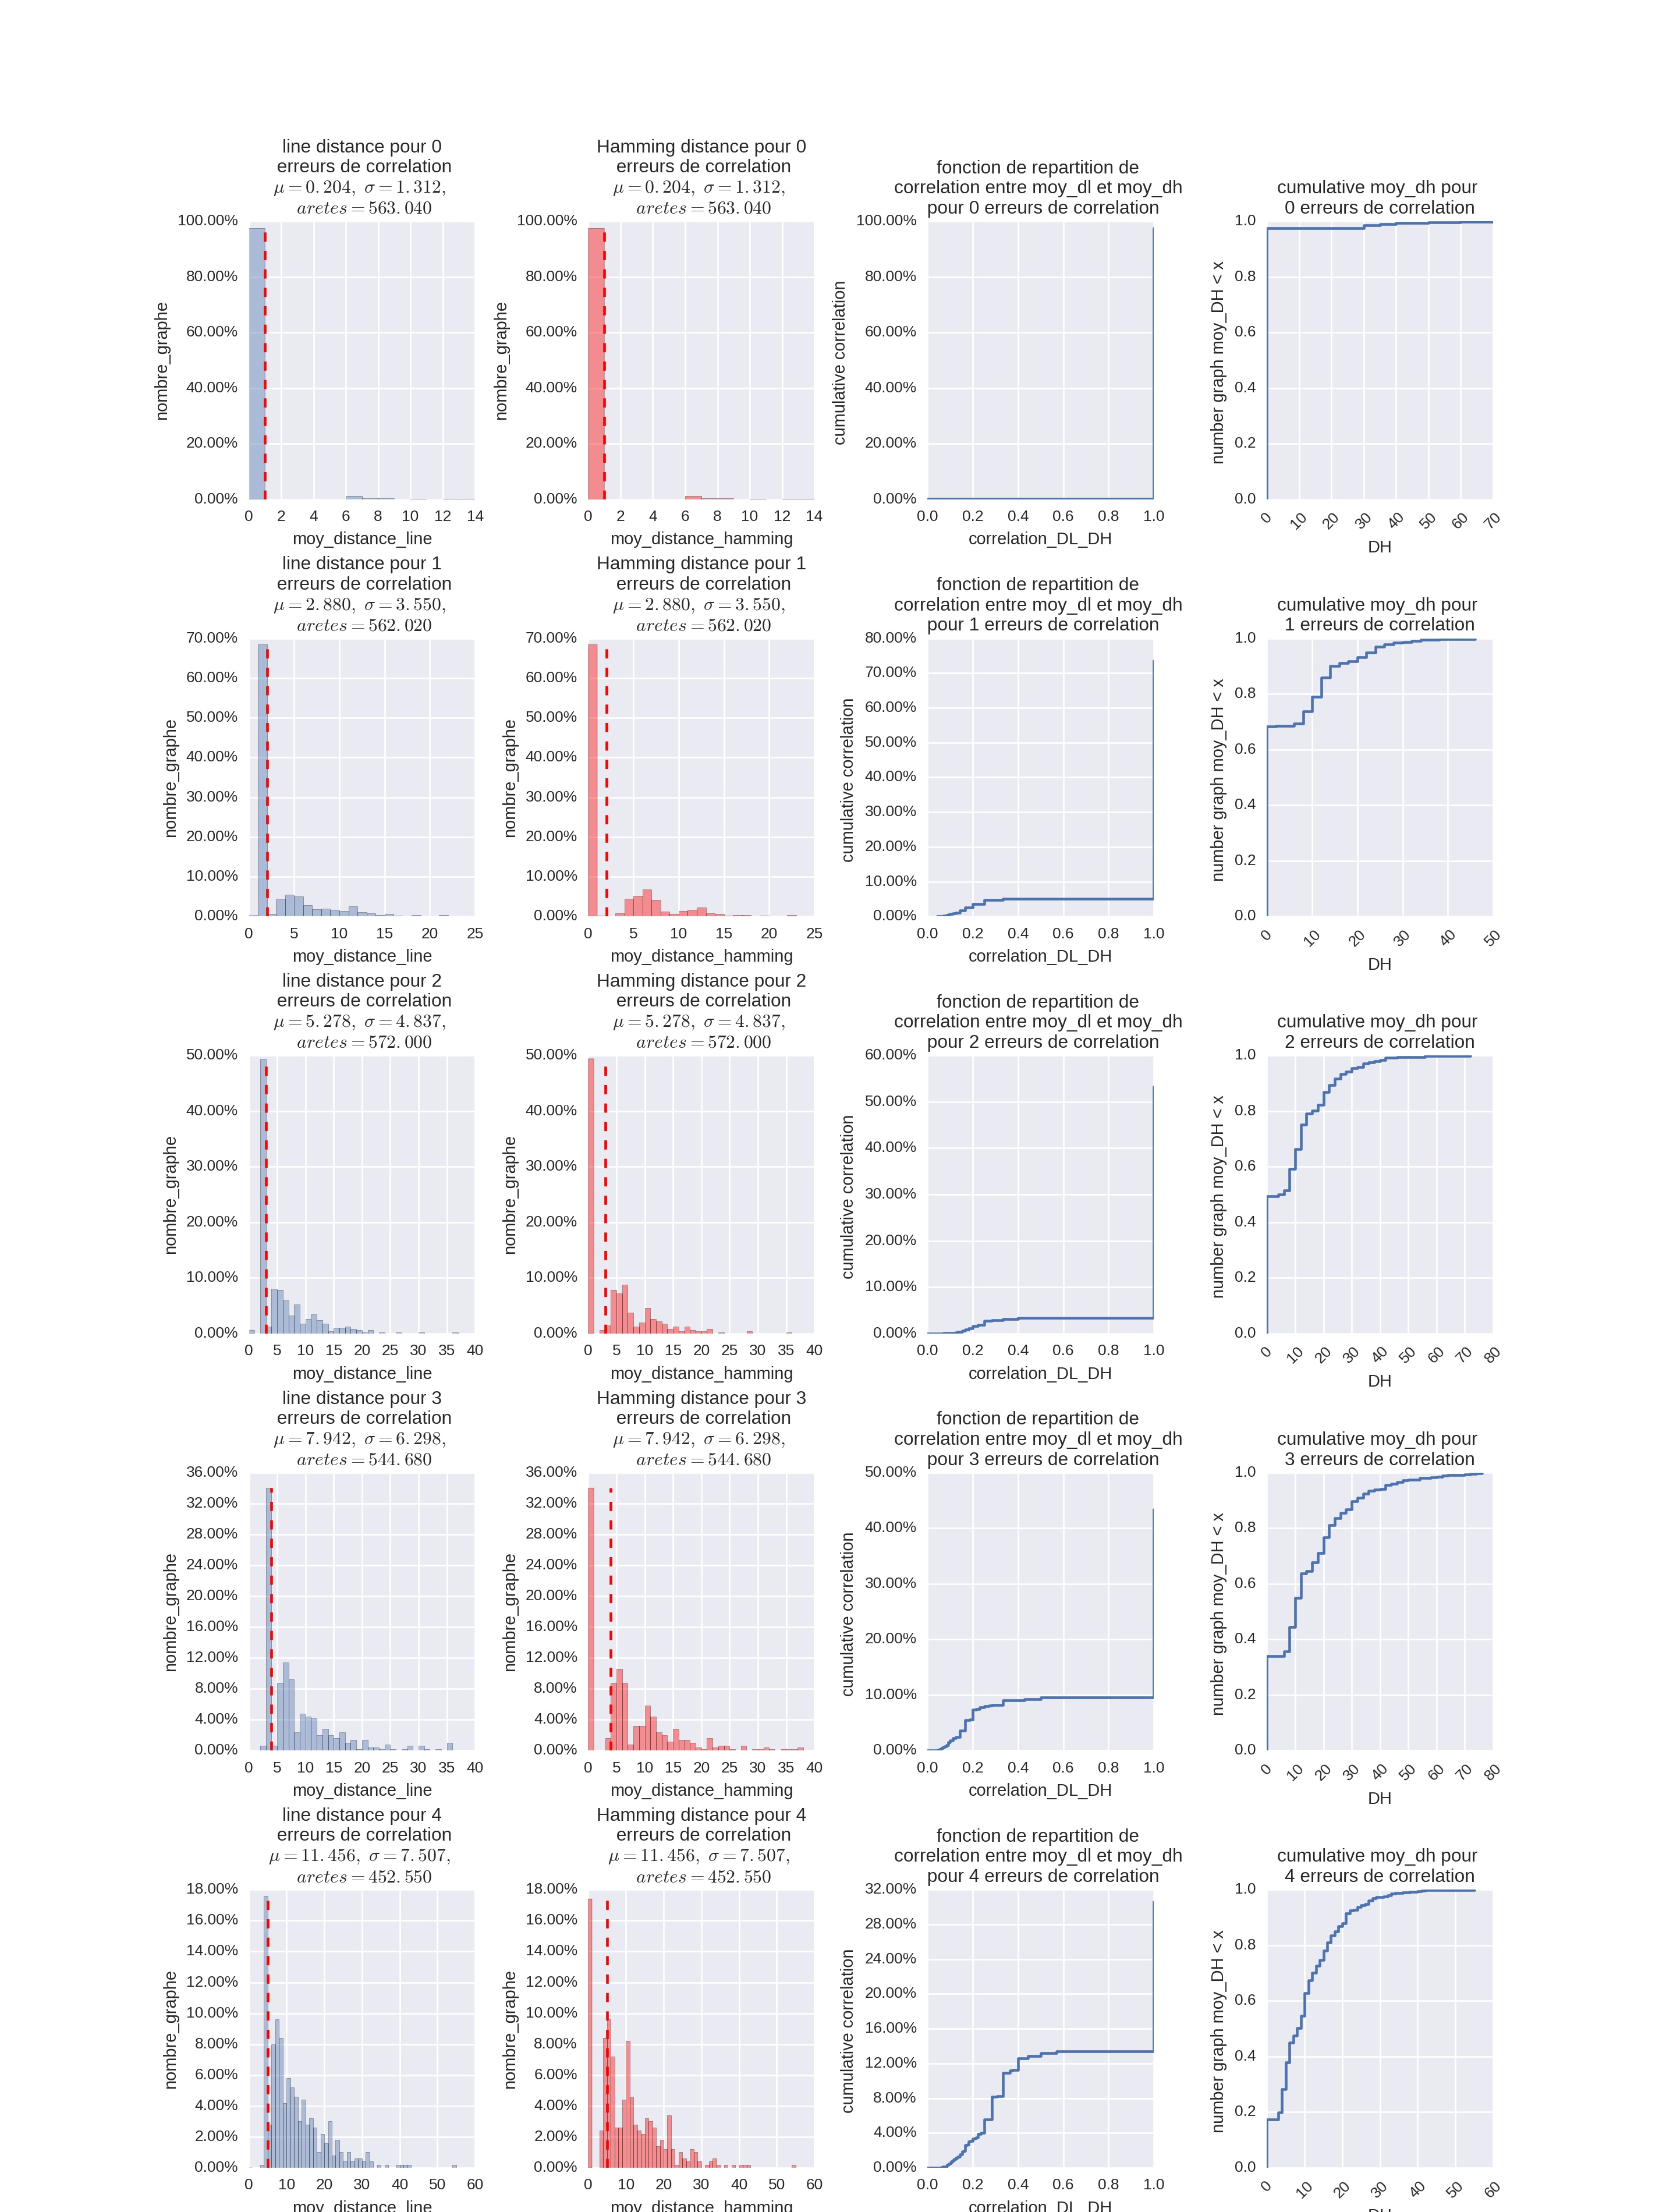
\includegraphics[width=550pt, height=600pt]{permut_distanceMoyenDLDH_k_0_4_aleatoire_p_05.jpeg}
%\caption{ M\'ethode de permutation al\'eatoire avec une fonction de correction \`a co\^ut unitaire : distribution des distances line $moy\_DL$ et de Hamming $moy\_DH$ pour $k \in [0,  5]$ corr\'elations alter\'ees}
%\label{permut_distanceMoyenDLDH_k_0_5_aleatoire_p_05} 
%\end{figure}

\begin{figure}[htb!] 
\centering
\includegraphics[width=500pt,height=160pt]{simulation_distanceMoyenDLDH_k_0_aleatoire_p_05.jpeg}
\caption{ M\'ethode de permutation al\'eatoire avec une fonction de correction \`a co\^ut unitaire : distribution des distances line $moy\_DL$ et de Hamming $moy\_DH$ pour $k =0 $ corr\'elation alter\'e}
\label{permut_distanceMoyenDLDH_k_0_aleatoire_p_05} 
\end{figure}

\begin{figure}[htb!] 
\centering
\includegraphics[width=550pt,height=600pt]{permut_distanceMoyenDLDH_k_1_2_5_9_aleatoire_p_05.jpeg}
\caption{ M\'ethode de permutation al\'eatoire avec une fonction de correction \`a co\^ut unitaire : distribution des distances line $moy\_DL$ et de Hamming $moy\_DH$ pour $k \in [1,2,5, 9]$ corr\'elations alter\'ees}
\label{permut_distanceMoyenDLDH_k_1_2_5_9_aleatoire_p_05} 
\end{figure}

%\begin{figure}[htb!] 
%\centering
%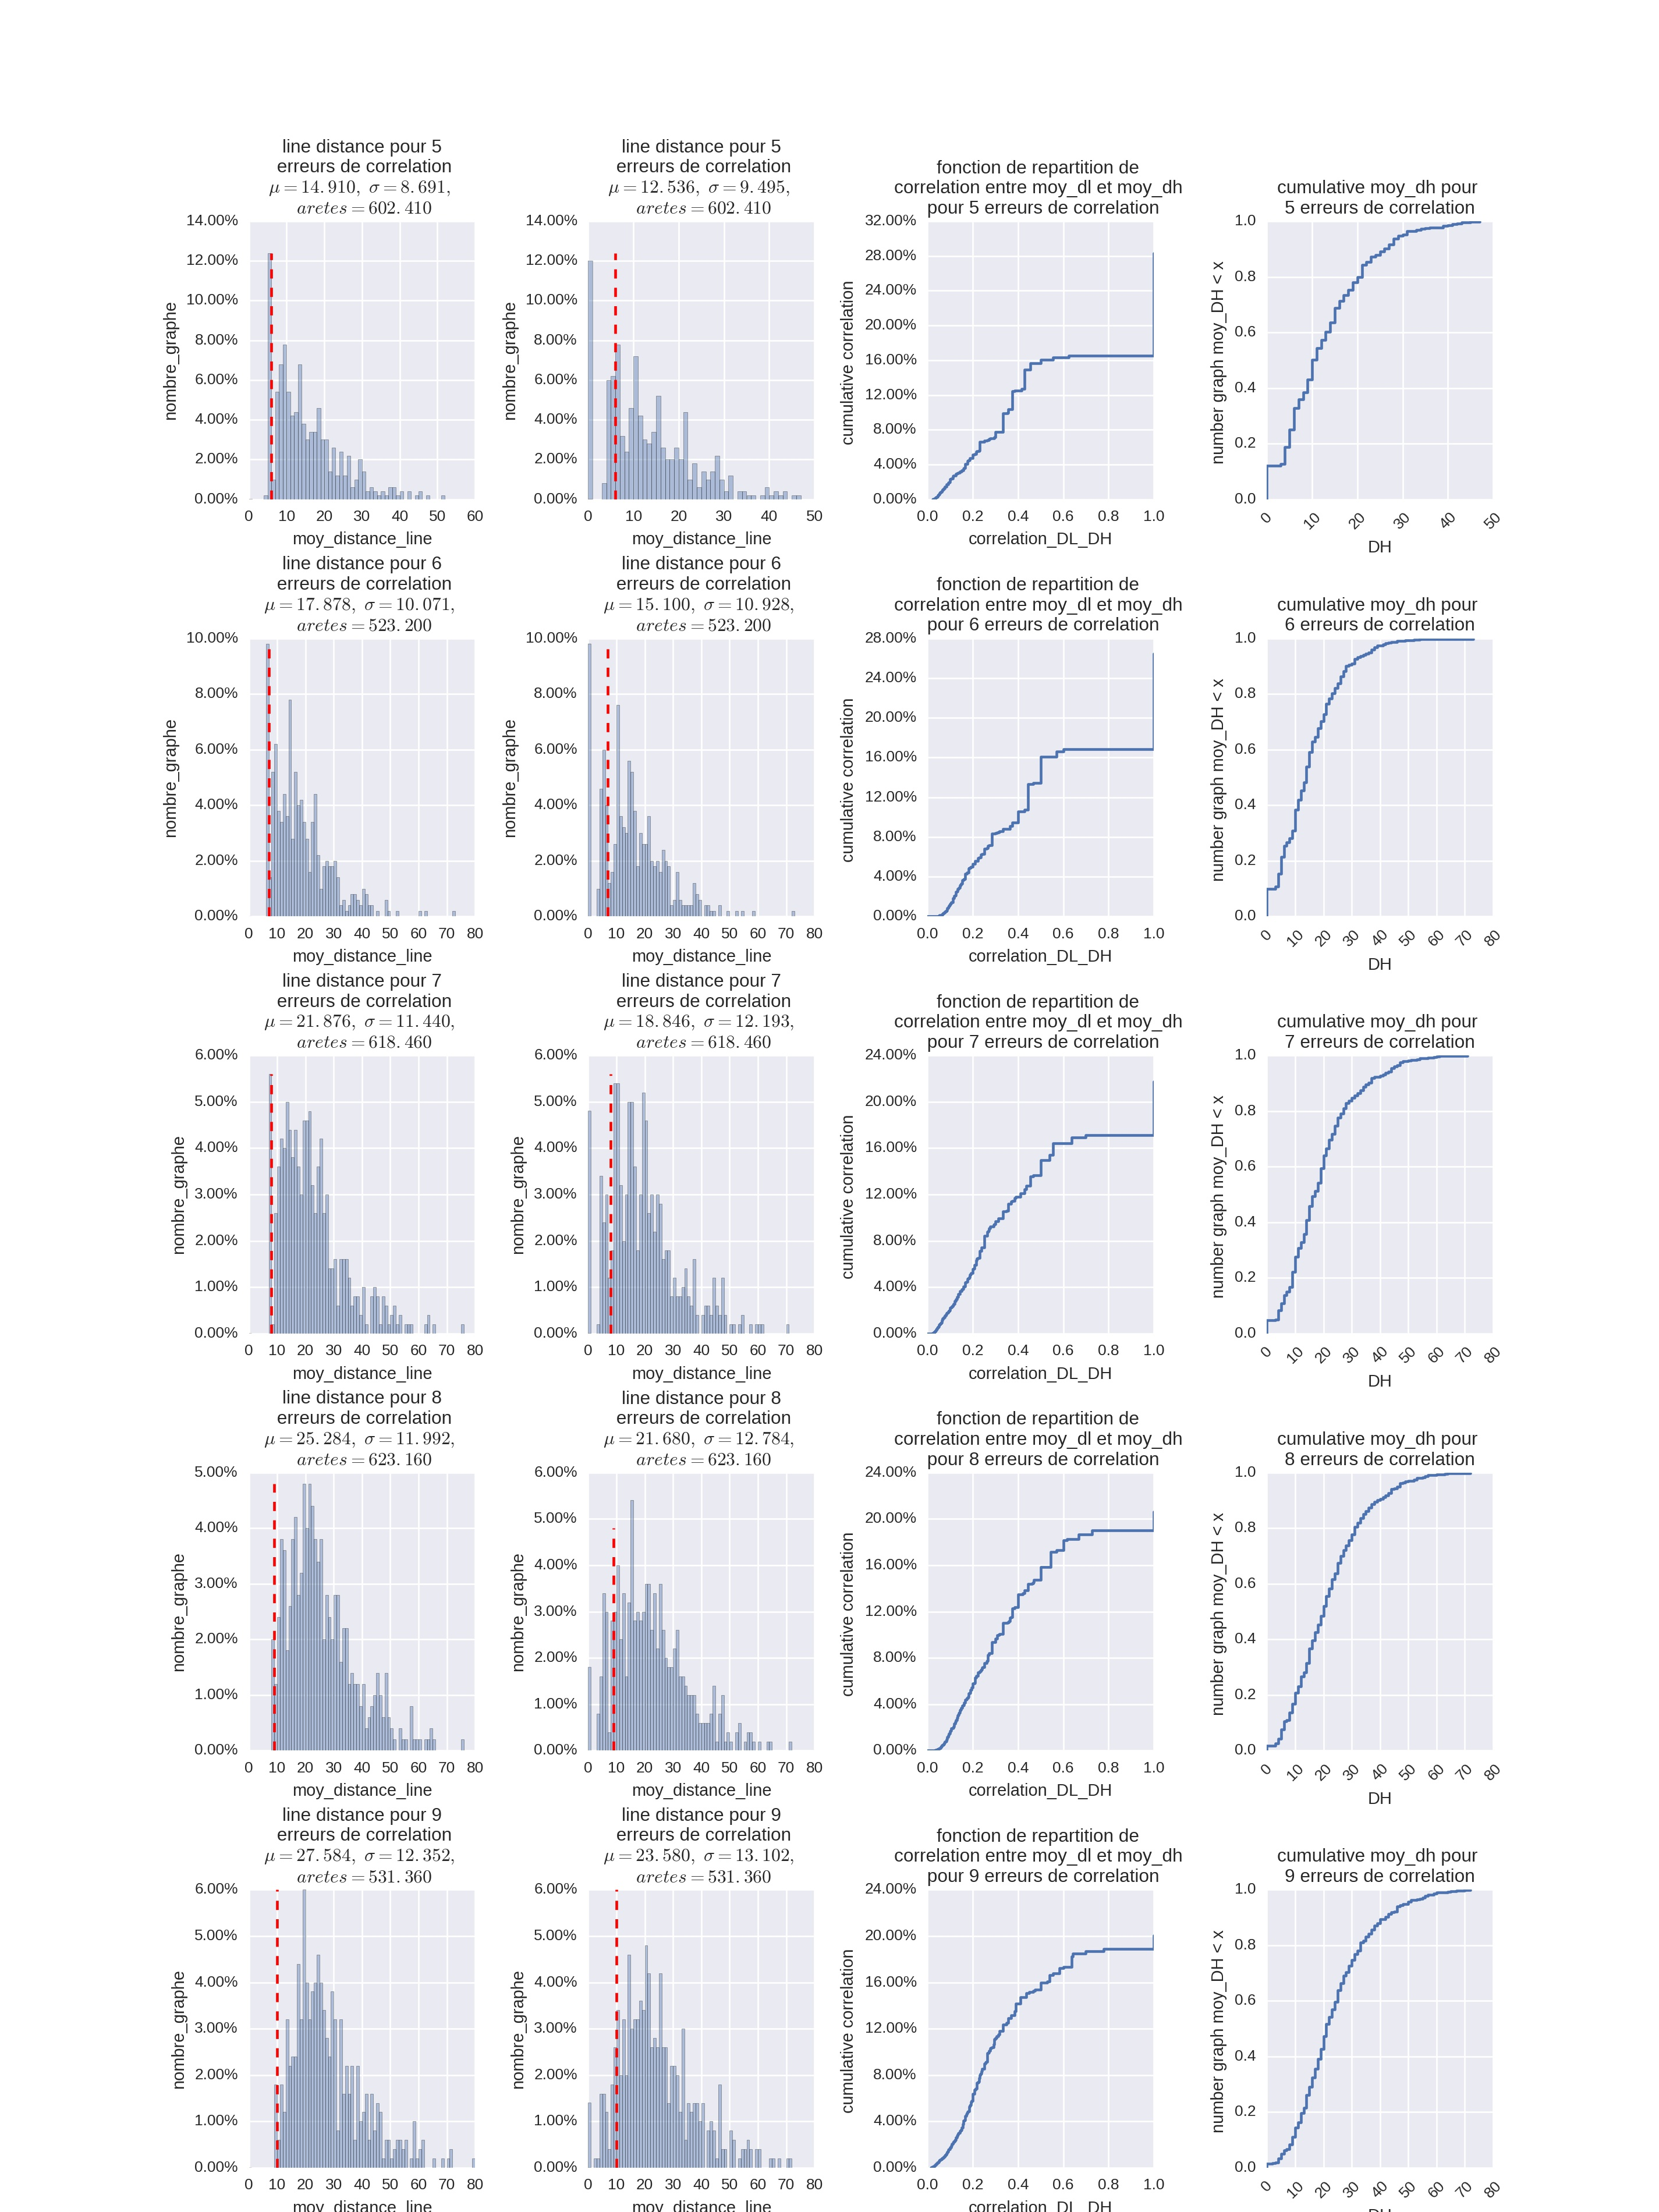
\includegraphics[width=550pt,height=600pt]{permut_distanceMoyenDLDH_k_5_9_aleatoire_p_05.jpeg}
%\caption{ M\'ethode de permutation al\'eatoire avec une fonction de correction \`a co\^ut unitaire : distribution des distances line $moy\_DL$ et de Hamming $moy\_DH$ pour $k \in [6,  9]$ corr\'elations alter\'ees}
%\label{permut_distanceMoyenDLDH_k_5_9_aleatoire_p_05} 
%\end{figure}

La figure \ref{permut_distanceMoyenDLDH_k_1_2_5_9_aleatoire_p_05} repr\'esente les distributions des distances line, de Hamming, des fonctions de r\'epartition de la corr\'elation entre les distances line et  de Hamming pour $k \in [1,2,5,9]$ erreurs. 
\newline
Pour $k=0$ erreur (figure \ref{permut_distanceMoyenDLDH_k_0_aleatoire_p_05}), nous avons un batonnet sur les histogrammes de distances line et de Hamming. Ce batonnet est le pourcentage d'ar\^etes identiques entre les graphes $G_k$ et $LG_k$ (distance line) et aussi entre les graphes  $LG$ et $LG_k$ (distance de Hamming). Nous remarquons que le pourcentage d'ar\^etes identiques est de $100\%$ et cela signifie que les graphes $LG_k$ et $LG$ sont isomorphes en ar\^etes c'est-\`a-dire que les ar\^etes des graphes $LG_k$ et $LG$ sont identiques. Ce qui est normal parce que nous n'avons ajout\'e aucune erreur dans le line-graphe $LG$. 
Par ailleurs, nous avons deux fonctions de r\'epartition. La premi\`ere fonction $y_{correlDLDH}^{0}$ calcule la corr\'elation entre les distances line et de Hamming. Elle est d\'efinie par l'\'equation \ref{eqCorrelMoyDLDH} et se localise dans la troisi\`eme colonne de la figure \ref{permut_distanceMoyenDLDH_k_1_2_5_9_aleatoire_p_05}. La deuxi\`eme fonction $y_{cumulDH}^{0}$, d\'efinie par l'\'equation \ref{eqCumulMoyDH}, calcule les corr\'elations cumul\'ees des distances de Hamming et occupe la quatri\`eme colonne de la figure \ref{permut_distanceMoyenDLDH_k_1_2_5_9_aleatoire_p_05}.
\begin{equation}
\label{eqCorrelMoyDLDH}
y_{correlDLDH}^{0} = \left\{
	\begin{aligned}
	0 \hspace{1 em} si \hspace{1 em} x < 1 \\
	100  \hspace{1 em}  si  \hspace{1 em}  x = 1
	\end{aligned}
	\right.
\end{equation}
\begin{equation}
\label{eqCumulMoyDH}
y_{cumulDH}^{0} = 1  \hspace{1 em}  si  \hspace{1 em}   x \in [0,1]
\end{equation}
La variable $x$ est la corr\'elation entre la distance line et la distance de Hamming.
En effet,  $x = 1$ implique que $DL = k$ et $DH = 0$ tandis que  $x = 0$ implique que $DL = k$ et $DH = k$.
L'\'equation  \ref{eqCorrelMoyDLDH} s'interpr\`ete comme suit : $y_{correlDLDH}^{0} = 100\%$ des line-graphes ont leur distance line et de Hamming correl\'ees ($x = 1$).
Le cas de $k=0$ erreur servira de r\'ef\'erence pour la meilleure performance de nos algorithmes.
\newline
%-- pour k \in [1,2]
Pour $k \in [1,2]$, dans la premi\`ere et seconde colonne, le batonnet de pic maximal est \`a gauche de la droite $y = k$ (droite en rouge) de chaque histogramme et  son pourcentage est sup\'erieur \`a $50 \%$. Les autres batonnets sont regroup\'es \`a droite de $y = k$ et le pic maximal du pourcentage de ces batonnets est inf\'erieur \`a $10\%$. La droite $y = k$ d\'esigne le nombre d'erreurs ajout\'ees dans le graphe de corr\'elation $G_k$.
Dans la seconde colonne, le pic correspond \`a $moy\_DH = 0$ ar\^ete indiquant qu'il n'y a aucune diff\'erence d'ar\^etes entre les  graphes $G_k$ et $LG_k$. Dans la premi\`ere colonne, le pic correspond \`a $k$ erreurs et son pourcentage est identique \`a celui de $k=0$ dans la seconde colonne. Cela signifie que les $k$ erreurs ajout\'ees dans $G_k$ ont \'et\'e supprim\'ees. Ainsi, nous retrouvons le line-graphe initial dans un cas sur deux lorsque nous ajoutons $k \le 2$ erreurs.
% par ailleurs comment se comporte les algos lorsque les k erreurs ne sont pas corrigees
Cependant, on observe que les distances line et de Hamming  ont approximativement les m\^emes valeurs lorsque les $k$ erreurs n'ont pas \'et\'e corrig\'ees. 
En effet, pour $x > 0.3$, $y_{correlDLDH}^{k} > 60\%$ et  pour $x \le 0.3$, $y_{correlDLDH}^{k} < 5\%$ (voir troisi\`eme colonne figure \ref{permut_distanceMoyenDLDH_k_1_2_5_9_aleatoire_p_05}). Or $y_{correlDLDH}^{k} \rightarrow 0\%$ signifie que $DL$ est \'egale \`a $k$ ($DL = k$) et $DH$ tend vers $k$ ($DH \rightarrow k$). Donc $y_{correlDLDH}^{k} < 5\%$ implique que $DL = k$ et $DH \approx k$.
Ainsi, les distances line et de hamming sont corr\'el\'ees dans $5\%$ des line-graphes et le line-graphe $LG_k$, d\'ecouvert par les algorithmes, devient  au line-graphe initial $LG$ si nous retirons/ajout\'ons les $DL$ ar\^etes du graphe $LG_k$.
\newline
%-- pour k \in [5,9] 
Pour $k  = 5$ erreurs,  le pic de chaque histogramme baisse significativement $nombre\_graphe \approx 12 \%$ et se localise toujours $moy\_distance\_line = k$, \`a la gauche de la droite $y = k$ (voir colonnes 1 et 2 dans la figure \ref{permut_distanceMoyenDLDH_k_1_2_5_9_aleatoire_p_05}). 
Toutefois, la distribution \`a la droite de la droite  $y = k$ est plus \'elev\'ee par rapport \`a celle \`a la gauche de la droite.
Les $12\%$ des line-graphes $LG_k$ isomorphes en ar\^etes \`a $LG$ s'expliquent  par le type d'erreurs et par l'emplacement des erreurs dans le graphe $G_k$. En effet, ces erreurs sont des corr\'elations {\em fausses n\'egatives} et ces ar\^etes supprim\'ees n'appartiennent pas \`a des cliques voisines.
Cependant, quelque soit le type d'erreurs, nos algorithmes ajoutent beaucoup ar\^etes pour obtenir le line-graphe $LG_k$ lorsque les erreurs sont h\'et\'erog\`enes. Par exemple, nous avons $10$, $20$ ar\^etes diff\'erentes  pour $5$ erreurs ajout\'ees.
\newline
%-- pour k \in [9]
De m\^eme, le ph\'enom\`ene est identique pour $k  = 9$ erreurs et la particularit\'e de la distribution est l'absence de batonnets \`a la gauche de la droite $y = k$ (voir colonnes 1, derni\`ere ligne dans la figure \ref{permut_distanceMoyenDLDH_k_1_2_5_9_aleatoire_p_05}).
Le pic est \`a $moy\_distance\_line = 23$ avec une valeur de $nombre\_graphe \approx 6 \%$.
Nous remarquons que moins de $3\%$ des line-graphes $LG_k$ sont isomorphes  en ar\^etes \`a $LG$ c'est-\`a-dire la corr\'elation entre les distances line et de hamming est de $1$ (voir la troisi\`eme colonne de la figure \ref{permut_distanceMoyenDLDH_k_1_2_5_9_aleatoire_p_05}). 
Les autres line-graphes $LG_k$ ont leur corr\'elation entre les distances line et de Hamming qui tend vers $0$.  C'est pourquoi, pour $k=9$, les courbes de  $y_{correlDLDH}^{k}$ et $y_{cumulDH}^{k}$ ont cette forme enrob\'ee proche de la fonction  sigmoide de param\^etre $\lambda \le -15$  et sont diff\'erentes de celles de $k=0$, notre cas de r\'ef\'erence. Pour rappel, pr\'ecisons que ces courbes  tendent la fonction suivante $f_{\lambda}(x) = \frac{1}{1+e^{\lambda * (x-0.5)}}$.\newline
Les erreurs de corr\'elations $k \in [1,9]$ sont pr\'esent\'ees dans les figures \ref{permut_distanceMoyenDLDH_k_0_5_aleatoire_p_05} et  \ref{permut_distanceMoyenDLDH_k_5_9_aleatoire_p_05}) de l'annexe \ref{annexe_distribution_0_9}.
\newline
Bien que les distributions de distance line et de Hamming soient asym\'etriques (pour $k < 5$), sym\'etriques (pour $k>6$) et que certaines distances line et de Hamming soient identiques, nous interrogent sur l'\'evolution des distributions des distances line par rapport \`a celles de Hamming. 


%Pour $k \in [1,4]$, l'ensemble des batonnets, regroup\'es avant la droite $y = k$ (droite en rouge) de chaque histogramme, a un pourcentage sup\'erieure \`a $50 \%$. La pr\'esence de cette droite nous indique que, dans le majorit\'e des cas,  qu'il existe une diff\'erence de $k$ ar\^etes entre les graphes $G_k$ et $LG_k$ (voir distance line figure \ref{permut_distanceMoyenDLDH_k_0_5_aleatoire_p_05}) et ces $k$ ar\^etes correspondent aux erreurs ajout\'ees dans la matrice d'adjacence $matE$ du line-graphe $LG$. Cela explique 
%la distance de hamming de $0$ ar\^ete entre $LG$ et $LG_k$ et le pourcentage pour $0$ erreur est le pic de chaque histogramme (voir distance de Hamming figure \ref{permut_distanceMoyenDLDH_k_0_5_aleatoire_p_05}).

% ajouter les fonctions cumulatives

%Au d\'el\`a de $k \ge 5$ erreurs, le pic de chaque histogramme baisse significativement quand $k$ augmente (voir distances line et de  Hamming figure \ref{permut_distanceMoyenDLDH_k_5_9_aleatoire_p_05}). Une explication est la pr\'esence d'ar\^etes erron\'ees dans les line graphes $LG_k$ propos\'es parce que la majorit\'e de ces line-graphes qui ont plus de $k$ ar\^etes diff\'erentes entre $LG_k$ et $G_k$ alors que ce nombre $k$ doit correspondre au nombre d'erreurs ajout\'ees dans le line-graphe $LG$. Il s'illustre parfaitement avec $k = 9$ erreurs dans la figure \ref{permut_distanceMoyenDLDH_k_5_9_aleatoire_p_05} o\`u on a moins de $13\%$ de line-graphes dont les ar\^etes sont identiques et les $87\%$ restants ont plus d'une  ar\^ete diff\'erente.
%\newline
%-------
%Par ailleurs, les fonctions de r\'epartition des corr\'elations entre distances line et de Hamming et celle de la distance de Hamming ont des courbes  qui s'eloignent de celle de $k = 0$ erreur. En effet, ces courbes se divisent en deux parties : une courbe croissante et une droite verticale (distance de Hamming) ou horizontale (distance line). 
%Pour $k \in [1,4]$, dans les figures des distributions cumulatives des distances de Hamming (colonne 4 de la figure \ref{permut_distanceMoyenDLDH_k_5_9_aleatoire_p_05}), on remarque que la droite verticale pour $k$ erreurs baisse quand $k$ augmente. Cette droite est le pourcentage de line-graphes identiques ($LG$ et $LG_k$). Par exemple, on a $69\%$ de line-graphes $LG_k$ identiques \`a $LG$ pour $k = 1$ alors qu'on en a que $19\%$ pour $k=4$. Cela est d\^u \`a l'ajout d'ar\^etes dans $LG_k$ n'appartenant pas \`a $LG$. Il se  forme une courbe exponentielle croissante dans laquelle on a plus de $10$ ar\^etes diff\'erentes pour $k \le 5$.  \newline
%De m\^eme, au d\'el\`a du nombre d'ar\^etes diff\'erentes c'est-\`a-dire $moy\_DH > k$, nous constatons une droite verticale tr\`es courte qui baisse \'egalement quand la variable $moy\_DH$ augmente. Cela signifie qu'il y a tr\`es peu de line-graphes $LG_k$ ayant des  distances de Hamming tr\`es \'elev\'ees par rapport aux $k$ erreurs (voir figures \ref{permut_distanceMoyenDLDH_k_0_5_aleatoire_p_05} et \ref{permut_distanceMoyenDLDH_k_5_9_aleatoire_p_05})  pour $k \ge 5$.
%\newline
%Le fait que les distributions de distance line et de Hamming soient, toutes les deux, asym\'etriques (pour $k \le 6$) soient sym\'etriques (pour $k>6$) nous interrogent sur l'\'evolution des distributions des distances line par rapport \`a celles de Hamming. 